% Options for packages loaded elsewhere
\PassOptionsToPackage{unicode}{hyperref}
\PassOptionsToPackage{hyphens}{url}
\PassOptionsToPackage{dvipsnames,svgnames,x11names}{xcolor}
%
\documentclass[
  letterpaper,
  DIV=11,
  numbers=noendperiod]{scrartcl}

\usepackage{amsmath,amssymb}
\usepackage{iftex}
\ifPDFTeX
  \usepackage[T1]{fontenc}
  \usepackage[utf8]{inputenc}
  \usepackage{textcomp} % provide euro and other symbols
\else % if luatex or xetex
  \usepackage{unicode-math}
  \defaultfontfeatures{Scale=MatchLowercase}
  \defaultfontfeatures[\rmfamily]{Ligatures=TeX,Scale=1}
\fi
\usepackage{lmodern}
\ifPDFTeX\else  
    % xetex/luatex font selection
\fi
% Use upquote if available, for straight quotes in verbatim environments
\IfFileExists{upquote.sty}{\usepackage{upquote}}{}
\IfFileExists{microtype.sty}{% use microtype if available
  \usepackage[]{microtype}
  \UseMicrotypeSet[protrusion]{basicmath} % disable protrusion for tt fonts
}{}
\makeatletter
\@ifundefined{KOMAClassName}{% if non-KOMA class
  \IfFileExists{parskip.sty}{%
    \usepackage{parskip}
  }{% else
    \setlength{\parindent}{0pt}
    \setlength{\parskip}{6pt plus 2pt minus 1pt}}
}{% if KOMA class
  \KOMAoptions{parskip=half}}
\makeatother
\usepackage{xcolor}
\setlength{\emergencystretch}{3em} % prevent overfull lines
\setcounter{secnumdepth}{-\maxdimen} % remove section numbering
% Make \paragraph and \subparagraph free-standing
\ifx\paragraph\undefined\else
  \let\oldparagraph\paragraph
  \renewcommand{\paragraph}[1]{\oldparagraph{#1}\mbox{}}
\fi
\ifx\subparagraph\undefined\else
  \let\oldsubparagraph\subparagraph
  \renewcommand{\subparagraph}[1]{\oldsubparagraph{#1}\mbox{}}
\fi

\usepackage{color}
\usepackage{fancyvrb}
\newcommand{\VerbBar}{|}
\newcommand{\VERB}{\Verb[commandchars=\\\{\}]}
\DefineVerbatimEnvironment{Highlighting}{Verbatim}{commandchars=\\\{\}}
% Add ',fontsize=\small' for more characters per line
\usepackage{framed}
\definecolor{shadecolor}{RGB}{241,243,245}
\newenvironment{Shaded}{\begin{snugshade}}{\end{snugshade}}
\newcommand{\AlertTok}[1]{\textcolor[rgb]{0.68,0.00,0.00}{#1}}
\newcommand{\AnnotationTok}[1]{\textcolor[rgb]{0.37,0.37,0.37}{#1}}
\newcommand{\AttributeTok}[1]{\textcolor[rgb]{0.40,0.45,0.13}{#1}}
\newcommand{\BaseNTok}[1]{\textcolor[rgb]{0.68,0.00,0.00}{#1}}
\newcommand{\BuiltInTok}[1]{\textcolor[rgb]{0.00,0.23,0.31}{#1}}
\newcommand{\CharTok}[1]{\textcolor[rgb]{0.13,0.47,0.30}{#1}}
\newcommand{\CommentTok}[1]{\textcolor[rgb]{0.37,0.37,0.37}{#1}}
\newcommand{\CommentVarTok}[1]{\textcolor[rgb]{0.37,0.37,0.37}{\textit{#1}}}
\newcommand{\ConstantTok}[1]{\textcolor[rgb]{0.56,0.35,0.01}{#1}}
\newcommand{\ControlFlowTok}[1]{\textcolor[rgb]{0.00,0.23,0.31}{#1}}
\newcommand{\DataTypeTok}[1]{\textcolor[rgb]{0.68,0.00,0.00}{#1}}
\newcommand{\DecValTok}[1]{\textcolor[rgb]{0.68,0.00,0.00}{#1}}
\newcommand{\DocumentationTok}[1]{\textcolor[rgb]{0.37,0.37,0.37}{\textit{#1}}}
\newcommand{\ErrorTok}[1]{\textcolor[rgb]{0.68,0.00,0.00}{#1}}
\newcommand{\ExtensionTok}[1]{\textcolor[rgb]{0.00,0.23,0.31}{#1}}
\newcommand{\FloatTok}[1]{\textcolor[rgb]{0.68,0.00,0.00}{#1}}
\newcommand{\FunctionTok}[1]{\textcolor[rgb]{0.28,0.35,0.67}{#1}}
\newcommand{\ImportTok}[1]{\textcolor[rgb]{0.00,0.46,0.62}{#1}}
\newcommand{\InformationTok}[1]{\textcolor[rgb]{0.37,0.37,0.37}{#1}}
\newcommand{\KeywordTok}[1]{\textcolor[rgb]{0.00,0.23,0.31}{#1}}
\newcommand{\NormalTok}[1]{\textcolor[rgb]{0.00,0.23,0.31}{#1}}
\newcommand{\OperatorTok}[1]{\textcolor[rgb]{0.37,0.37,0.37}{#1}}
\newcommand{\OtherTok}[1]{\textcolor[rgb]{0.00,0.23,0.31}{#1}}
\newcommand{\PreprocessorTok}[1]{\textcolor[rgb]{0.68,0.00,0.00}{#1}}
\newcommand{\RegionMarkerTok}[1]{\textcolor[rgb]{0.00,0.23,0.31}{#1}}
\newcommand{\SpecialCharTok}[1]{\textcolor[rgb]{0.37,0.37,0.37}{#1}}
\newcommand{\SpecialStringTok}[1]{\textcolor[rgb]{0.13,0.47,0.30}{#1}}
\newcommand{\StringTok}[1]{\textcolor[rgb]{0.13,0.47,0.30}{#1}}
\newcommand{\VariableTok}[1]{\textcolor[rgb]{0.07,0.07,0.07}{#1}}
\newcommand{\VerbatimStringTok}[1]{\textcolor[rgb]{0.13,0.47,0.30}{#1}}
\newcommand{\WarningTok}[1]{\textcolor[rgb]{0.37,0.37,0.37}{\textit{#1}}}

\providecommand{\tightlist}{%
  \setlength{\itemsep}{0pt}\setlength{\parskip}{0pt}}\usepackage{longtable,booktabs,array}
\usepackage{calc} % for calculating minipage widths
% Correct order of tables after \paragraph or \subparagraph
\usepackage{etoolbox}
\makeatletter
\patchcmd\longtable{\par}{\if@noskipsec\mbox{}\fi\par}{}{}
\makeatother
% Allow footnotes in longtable head/foot
\IfFileExists{footnotehyper.sty}{\usepackage{footnotehyper}}{\usepackage{footnote}}
\makesavenoteenv{longtable}
\usepackage{graphicx}
\makeatletter
\def\maxwidth{\ifdim\Gin@nat@width>\linewidth\linewidth\else\Gin@nat@width\fi}
\def\maxheight{\ifdim\Gin@nat@height>\textheight\textheight\else\Gin@nat@height\fi}
\makeatother
% Scale images if necessary, so that they will not overflow the page
% margins by default, and it is still possible to overwrite the defaults
% using explicit options in \includegraphics[width, height, ...]{}
\setkeys{Gin}{width=\maxwidth,height=\maxheight,keepaspectratio}
% Set default figure placement to htbp
\makeatletter
\def\fps@figure{htbp}
\makeatother

\KOMAoption{captions}{tableheading}
\makeatletter
\@ifpackageloaded{tcolorbox}{}{\usepackage[skins,breakable]{tcolorbox}}
\@ifpackageloaded{fontawesome5}{}{\usepackage{fontawesome5}}
\definecolor{quarto-callout-color}{HTML}{909090}
\definecolor{quarto-callout-note-color}{HTML}{0758E5}
\definecolor{quarto-callout-important-color}{HTML}{CC1914}
\definecolor{quarto-callout-warning-color}{HTML}{EB9113}
\definecolor{quarto-callout-tip-color}{HTML}{00A047}
\definecolor{quarto-callout-caution-color}{HTML}{FC5300}
\definecolor{quarto-callout-color-frame}{HTML}{acacac}
\definecolor{quarto-callout-note-color-frame}{HTML}{4582ec}
\definecolor{quarto-callout-important-color-frame}{HTML}{d9534f}
\definecolor{quarto-callout-warning-color-frame}{HTML}{f0ad4e}
\definecolor{quarto-callout-tip-color-frame}{HTML}{02b875}
\definecolor{quarto-callout-caution-color-frame}{HTML}{fd7e14}
\makeatother
\makeatletter
\makeatother
\makeatletter
\makeatother
\makeatletter
\@ifpackageloaded{caption}{}{\usepackage{caption}}
\AtBeginDocument{%
\ifdefined\contentsname
  \renewcommand*\contentsname{Table of contents}
\else
  \newcommand\contentsname{Table of contents}
\fi
\ifdefined\listfigurename
  \renewcommand*\listfigurename{List of Figures}
\else
  \newcommand\listfigurename{List of Figures}
\fi
\ifdefined\listtablename
  \renewcommand*\listtablename{List of Tables}
\else
  \newcommand\listtablename{List of Tables}
\fi
\ifdefined\figurename
  \renewcommand*\figurename{Figure}
\else
  \newcommand\figurename{Figure}
\fi
\ifdefined\tablename
  \renewcommand*\tablename{Table}
\else
  \newcommand\tablename{Table}
\fi
}
\@ifpackageloaded{float}{}{\usepackage{float}}
\floatstyle{ruled}
\@ifundefined{c@chapter}{\newfloat{codelisting}{h}{lop}}{\newfloat{codelisting}{h}{lop}[chapter]}
\floatname{codelisting}{Listing}
\newcommand*\listoflistings{\listof{codelisting}{List of Listings}}
\makeatother
\makeatletter
\@ifpackageloaded{caption}{}{\usepackage{caption}}
\@ifpackageloaded{subcaption}{}{\usepackage{subcaption}}
\makeatother
\makeatletter
\@ifpackageloaded{tcolorbox}{}{\usepackage[skins,breakable]{tcolorbox}}
\makeatother
\makeatletter
\@ifundefined{shadecolor}{\definecolor{shadecolor}{rgb}{.97, .97, .97}}
\makeatother
\makeatletter
\makeatother
\makeatletter
\makeatother
\ifLuaTeX
  \usepackage{selnolig}  % disable illegal ligatures
\fi
\IfFileExists{bookmark.sty}{\usepackage{bookmark}}{\usepackage{hyperref}}
\IfFileExists{xurl.sty}{\usepackage{xurl}}{} % add URL line breaks if available
\urlstyle{same} % disable monospaced font for URLs
\hypersetup{
  pdftitle={Joining tables with dplyr},
  pdfauthor={Emily Malcolm-White},
  colorlinks=true,
  linkcolor={blue},
  filecolor={Maroon},
  citecolor={Blue},
  urlcolor={Blue},
  pdfcreator={LaTeX via pandoc}}

\title{Joining tables with \texttt{dplyr}}
\author{Emily Malcolm-White}
\date{}

\begin{document}
\maketitle
\ifdefined\Shaded\renewenvironment{Shaded}{\begin{tcolorbox}[interior hidden, borderline west={3pt}{0pt}{shadecolor}, boxrule=0pt, frame hidden, enhanced, sharp corners, breakable]}{\end{tcolorbox}}\fi

\hypertarget{nycflights23-dataset}{%
\section{\texorpdfstring{\texttt{nycflights23}
dataset}{nycflights23 dataset}}\label{nycflights23-dataset}}

\begin{Shaded}
\begin{Highlighting}[]
\CommentTok{\#LOAD PACKAGES}
\FunctionTok{library}\NormalTok{(tidyverse)}

\CommentTok{\#LOAD DATA}
\FunctionTok{library}\NormalTok{(nycflights23)}
\FunctionTok{data}\NormalTok{(}\StringTok{"flights"}\NormalTok{)}
\end{Highlighting}
\end{Shaded}

\texttt{nycflights23} contains information about all 435352 flights
departing NYC in 2023.

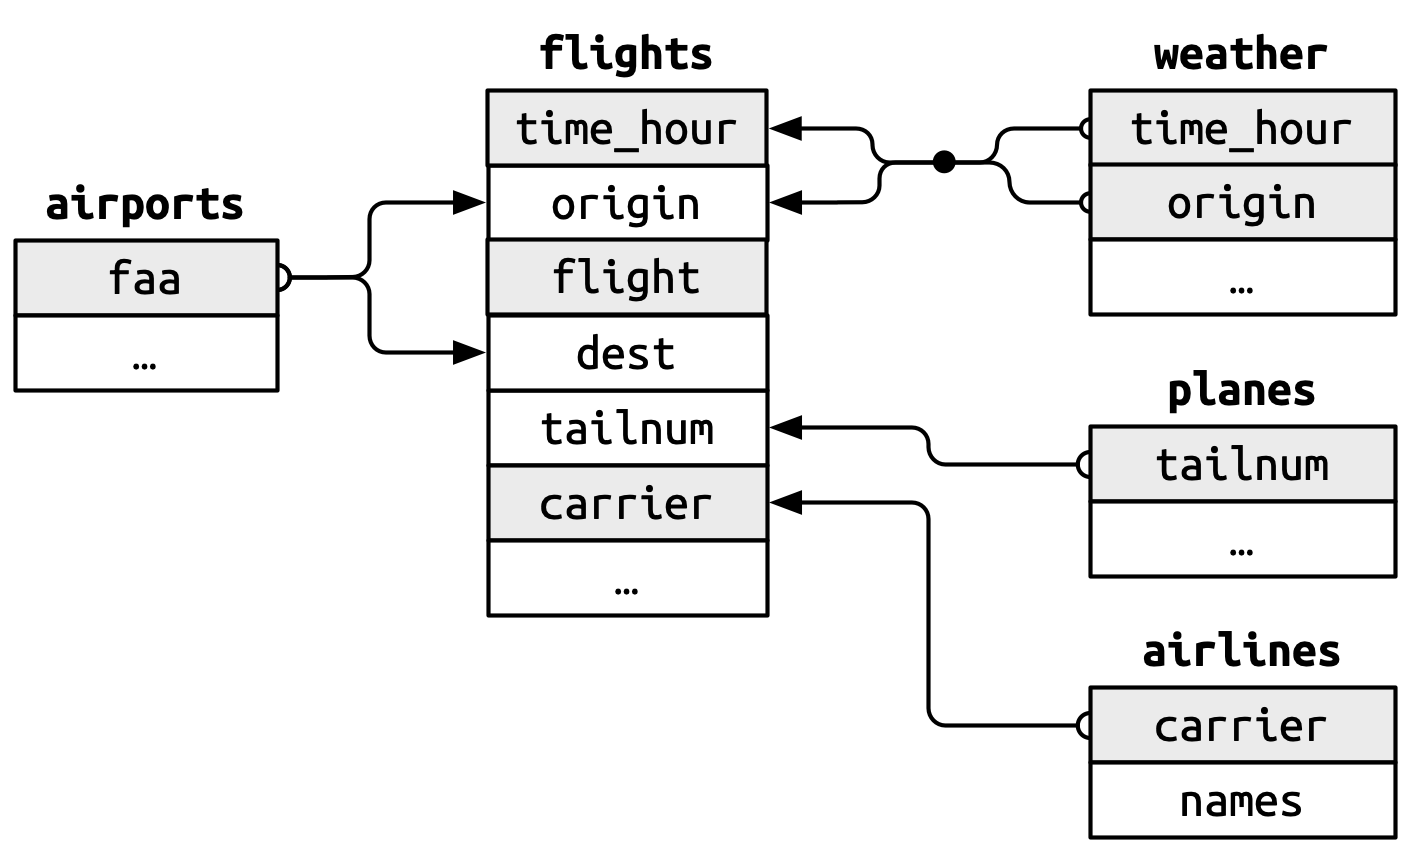
\includegraphics{118_I_joining_files/mediabag/relational.png}

\hypertarget{join-dataframes}{%
\section{Join dataframes}\label{join-dataframes}}

\hypertarget{matching-key-variable-names}{%
\subsection{Matching key variable
names}\label{matching-key-variable-names}}

Some airline names might be easy to guess (ie. ``UA'' is United
Airlines), but what airlines have the code ``VX'', ``HA'', and ``B6''?
Data on airline codes is provided in a dataset called \texttt{airlines}.

\begin{Shaded}
\begin{Highlighting}[]
\CommentTok{\#data("airlines")}
\end{Highlighting}
\end{Shaded}

We want to have all this information in one data frame instead of two
separate data frames.

The variable \texttt{carrier} in \texttt{flights} match the variable
\texttt{carrier} in the \texttt{airlines} dataset -- this is our
\emph{key variable}. In this case, they have the same name, but this
doesn't necessarily have to be true.

\begin{Shaded}
\begin{Highlighting}[]
\NormalTok{flights\_joined }\OtherTok{\textless{}{-}}\NormalTok{ flights }\SpecialCharTok{\%\textgreater{}\%} 
  \FunctionTok{inner\_join}\NormalTok{(airlines, }\AttributeTok{by=}\StringTok{"carrier"}\NormalTok{)}
\end{Highlighting}
\end{Shaded}

\hypertarget{different-key-variable-names}{%
\subsection{Different key variable
names}\label{different-key-variable-names}}

Say instead you are interested in the destinations of all domestic
flights departing NYC in 2013, and you ask yourself questions like:
``What cities are these airports in?'', or ``Is''ORD'' Orlando?''

\begin{Shaded}
\begin{Highlighting}[]
\FunctionTok{data}\NormalTok{(}\StringTok{"airports"}\NormalTok{)}
\end{Highlighting}
\end{Shaded}

In \texttt{airports} the airport code is in \texttt{faa}, whereas in
\texttt{flights} the airport codes are in \texttt{origin} and
\texttt{dest}.

\begin{Shaded}
\begin{Highlighting}[]
\NormalTok{flights\_with\_airport\_names }\OtherTok{\textless{}{-}}\NormalTok{ flights }\SpecialCharTok{\%\textgreater{}\%} 
  \FunctionTok{inner\_join}\NormalTok{(airports, }\AttributeTok{by =} \FunctionTok{c}\NormalTok{(}\StringTok{"dest"} \OtherTok{=} \StringTok{"faa"}\NormalTok{))}
\end{Highlighting}
\end{Shaded}

Let's construct the chain of pipe operators \%\textgreater\% that
computes the number of flights from NYC to each destination, but also
includes information about each destination airport:

\begin{Shaded}
\begin{Highlighting}[]
\NormalTok{named\_dests }\OtherTok{\textless{}{-}}\NormalTok{ flights }\SpecialCharTok{\%\textgreater{}\%}
  \FunctionTok{group\_by}\NormalTok{(dest) }\SpecialCharTok{\%\textgreater{}\%}
  \FunctionTok{summarize}\NormalTok{(}\AttributeTok{num\_flights =} \FunctionTok{n}\NormalTok{()) }\SpecialCharTok{\%\textgreater{}\%}
  \FunctionTok{arrange}\NormalTok{(}\FunctionTok{desc}\NormalTok{(num\_flights)) }\SpecialCharTok{\%\textgreater{}\%}
  \FunctionTok{inner\_join}\NormalTok{(airports, }\AttributeTok{by =} \FunctionTok{c}\NormalTok{(}\StringTok{"dest"} \OtherTok{=} \StringTok{"faa"}\NormalTok{)) }\SpecialCharTok{\%\textgreater{}\%}
  \FunctionTok{rename}\NormalTok{(}\AttributeTok{airport\_name =}\NormalTok{ name)}
\NormalTok{named\_dests}
\end{Highlighting}
\end{Shaded}

\begin{verbatim}
# A tibble: 114 x 9
   dest  num_flights airport_name             lat    lon   alt    tz dst   tzone
   <chr>       <int> <chr>                  <dbl>  <dbl> <dbl> <dbl> <chr> <chr>
 1 BOS         19036 General Edward Lawren~  42.4  -71.0    20    -5 A     Amer~
 2 ORD         18200 Chicago O'Hare Intern~  42.0  -87.9   672    -6 A     Amer~
 3 MCO         17756 Orlando International~  28.4  -81.3    96    -5 A     Amer~
 4 ATL         17570 Hartsfield Jackson At~  33.6  -84.4  1026    -5 A     Amer~
 5 MIA         16076 Miami International A~  25.8  -80.3     8    -5 A     Amer~
 6 LAX         15968 Los Angeles Internati~  33.9 -118.    125    -8 A     Amer~
 7 FLL         14239 Fort Lauderdale Holly~  26.1  -80.2     9    -5 A     Amer~
 8 CLT         12866 Charlotte Douglas Int~  35.2  -80.9   748    -5 A     Amer~
 9 DFW         11675 Dallas Fort Worth Int~  32.9  -97.0   607    -6 A     Amer~
10 SFO         11651 San Francisco Interna~  37.6 -122.     13    -8 A     Amer~
# i 104 more rows
\end{verbatim}

\hypertarget{multiple-key-variables}{%
\subsection{Multiple Key variables}\label{multiple-key-variables}}

In order to join the flights and weather data frames, we need more than
one key variable: \texttt{year}, \texttt{month}, \texttt{day},
\texttt{hour}, and \texttt{origin}. This is because the combination of
these 5 variables act to uniquely identify each observational unit in
the weather data frame: hourly weather recordings at each of the 3 NYC
airports.

\begin{Shaded}
\begin{Highlighting}[]
\FunctionTok{data}\NormalTok{(}\StringTok{"weather"}\NormalTok{)}
\end{Highlighting}
\end{Shaded}

\begin{Shaded}
\begin{Highlighting}[]
\NormalTok{flights\_weather\_joined }\OtherTok{\textless{}{-}}\NormalTok{ flights }\SpecialCharTok{\%\textgreater{}\%}
  \FunctionTok{inner\_join}\NormalTok{(weather, }\AttributeTok{by =} \FunctionTok{c}\NormalTok{(}\StringTok{"year"}\NormalTok{, }\StringTok{"month"}\NormalTok{, }\StringTok{"day"}\NormalTok{, }\StringTok{"hour"}\NormalTok{, }\StringTok{"origin"}\NormalTok{))}
\end{Highlighting}
\end{Shaded}

\hypertarget{why-is-this-useful}{%
\subsection{Why is this useful?}\label{why-is-this-useful}}

Updating labels:

\begin{Shaded}
\begin{Highlighting}[]
\NormalTok{flights }\SpecialCharTok{\%\textgreater{}\%} 
\FunctionTok{ggplot}\NormalTok{(}\FunctionTok{aes}\NormalTok{(}\AttributeTok{x =}\NormalTok{ carrier, }\AttributeTok{fill =}\NormalTok{ origin)) }\SpecialCharTok{+}
  \FunctionTok{geom\_bar}\NormalTok{() }\SpecialCharTok{+} 
  \FunctionTok{coord\_flip}\NormalTok{()}
\end{Highlighting}
\end{Shaded}

\begin{figure}[H]

{\centering 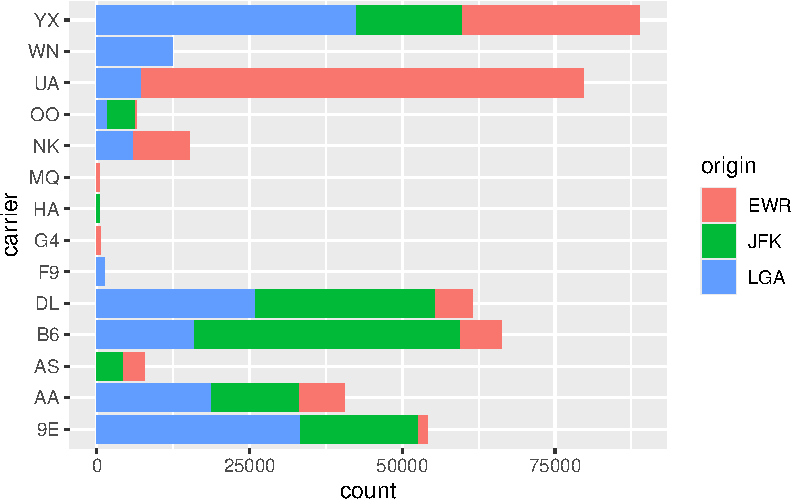
\includegraphics{118_I_joining_files/figure-pdf/unnamed-chunk-9-1.pdf}

}

\end{figure}

\begin{Shaded}
\begin{Highlighting}[]
\CommentTok{\#VS}

\NormalTok{flights }\SpecialCharTok{\%\textgreater{}\%} 
  \FunctionTok{inner\_join}\NormalTok{(airports, }\AttributeTok{by =} \FunctionTok{c}\NormalTok{(}\StringTok{"origin"} \OtherTok{=} \StringTok{"faa"}\NormalTok{)) }\SpecialCharTok{\%\textgreater{}\%} 
  \FunctionTok{rename}\NormalTok{(}\AttributeTok{origin\_airport =}\NormalTok{ name) }\SpecialCharTok{\%\textgreater{}\%} 
  \FunctionTok{inner\_join}\NormalTok{(airlines, }\AttributeTok{by =} \FunctionTok{c}\NormalTok{(}\StringTok{"carrier"}\NormalTok{)) }\SpecialCharTok{\%\textgreater{}\%}  
  \FunctionTok{rename}\NormalTok{(}\AttributeTok{carrier\_name=}\NormalTok{ name) }\SpecialCharTok{\%\textgreater{}\%} 
\FunctionTok{ggplot}\NormalTok{(}\AttributeTok{mapping =} \FunctionTok{aes}\NormalTok{(}\AttributeTok{x =}\NormalTok{ carrier\_name, }\AttributeTok{fill =}\NormalTok{ origin\_airport)) }\SpecialCharTok{+}
  \FunctionTok{geom\_bar}\NormalTok{() }\SpecialCharTok{+} 
  \FunctionTok{coord\_flip}\NormalTok{()}
\end{Highlighting}
\end{Shaded}

\begin{figure}[H]

{\centering 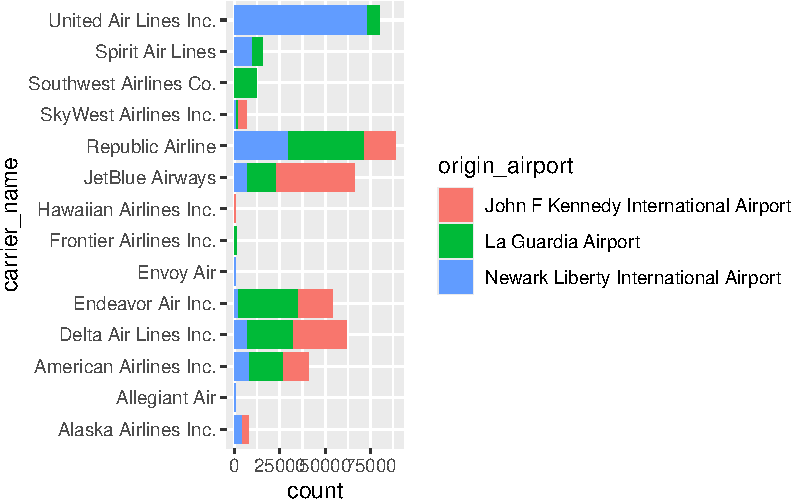
\includegraphics{118_I_joining_files/figure-pdf/unnamed-chunk-9-2.pdf}

}

\end{figure}

Exploring relationships between variables in separate tables:

\begin{Shaded}
\begin{Highlighting}[]
\NormalTok{flights\_weather\_joined }\SpecialCharTok{\%\textgreater{}\%} 
  \FunctionTok{filter}\NormalTok{(dep\_delay }\SpecialCharTok{\textgreater{}}\DecValTok{0}\NormalTok{) }\SpecialCharTok{\%\textgreater{}\%} 
  \FunctionTok{ggplot}\NormalTok{(}\FunctionTok{aes}\NormalTok{(}\AttributeTok{x=}\NormalTok{temp, }\AttributeTok{y=}\NormalTok{dep\_delay)) }\SpecialCharTok{+}
  \FunctionTok{geom\_point}\NormalTok{()}
\end{Highlighting}
\end{Shaded}

\begin{figure}[H]

{\centering 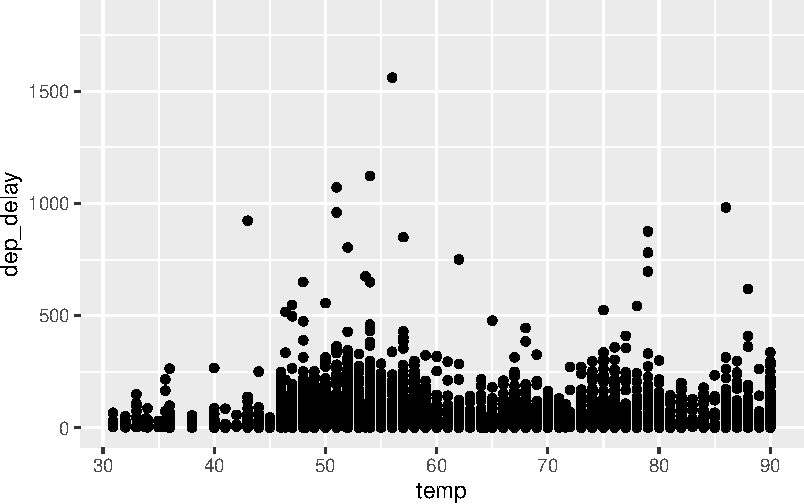
\includegraphics{118_I_joining_files/figure-pdf/unnamed-chunk-10-1.pdf}

}

\end{figure}

\hypertarget{different-types-of-joins}{%
\section{Different Types of Joins}\label{different-types-of-joins}}

\begin{figure}

{\centering 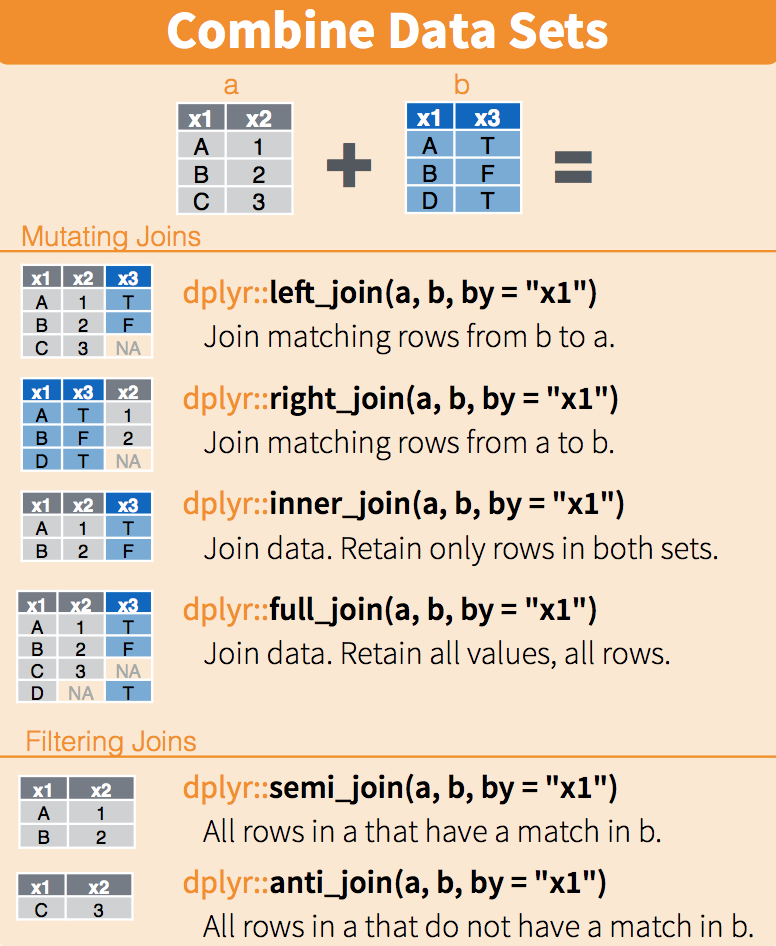
\includegraphics{118_I_joining_files/mediabag/joins.png}

}

\caption{Credit: RStudio}

\end{figure}

\hypertarget{common-issues-with-joining}{%
\section{Common Issues with Joining}\label{common-issues-with-joining}}

\begin{itemize}
\tightlist
\item
  duplicate keys
\item
  lowercase/uppercase
\item
  symbols or whitespace
\item
  Make sure the join fields are the same format.
\end{itemize}

\begin{tcolorbox}[enhanced jigsaw, left=2mm, rightrule=.15mm, leftrule=.75mm, opacityback=0, toprule=.15mm, arc=.35mm, colback=white, bottomrule=.15mm, breakable]

\textbf{External Resources}\vspace{2mm}

\begin{itemize}
\tightlist
\item
  \href{https://r4ds.hadley.nz/joins}{R for Data Science, Joins}
\end{itemize}

\end{tcolorbox}



\end{document}
